\documentclass[11pt]{article}
\usepackage[utf8]{inputenc}
\usepackage{amsmath}
\usepackage{amsfonts}
\usepackage{amssymb}
\usepackage{geometry}
\usepackage{enumitem}
\usepackage{graphicx}
\usepackage{tikz}
\usepackage{pgfplots}
\usepackage{amsthm}
\usepackage{mathtools}

\geometry{margin=1in}

\theoremstyle{definition}
\newtheorem{definition}{Definition}[section]
\newtheorem{theorem}{Theorem}[section]
\newtheorem{lemma}{Lemma}[section]
\newtheorem{corollary}{Corollary}[section]
\newtheorem{example}{Example}[section]
\newtheorem{proposition}{Proposition}[section]

\title{Optimization Theory Summary}
\author{Mathematical Notes}
\date{\today}

\begin{document}

\maketitle

\tableofcontents
\newpage

\section{Linear Programming}

\subsection{Standard Form}
\begin{definition}
A linear programming problem in standard form:
\begin{align}
\min \quad & c^T x \\
\text{s.t.} \quad & Ax = b \\
& x \geq 0
\end{align}
where $A \in \mathbb{R}^{m \times n}$, $b \in \mathbb{R}^m$, $c \in \mathbb{R}^n$.
\end{definition}

\subsection{Basic Solutions}
\begin{definition}
A \textbf{basic solution} is obtained by setting $n-m$ variables to zero and solving the resulting system. If all variables are nonnegative, it's a \textbf{basic feasible solution}.
\end{definition}

\subsection{Simplex Method}
\begin{definition}
The simplex method:
\begin{enumerate}
    \item Start with a basic feasible solution
    \item Choose entering variable (most negative reduced cost)
    \item Choose leaving variable (minimum ratio test)
    \item Pivot to new basic feasible solution
    \item Repeat until optimal
\end{enumerate}
\end{definition}

\subsection{Duality}
\begin{definition}
The dual of the primal problem $\min\{c^T x : Ax = b, x \geq 0\}$ is:
$$\max \quad b^T y \quad \text{s.t.} \quad A^T y \leq c$$
\end{definition}

\begin{theorem}[Strong Duality]
If the primal has an optimal solution, then so does the dual, and their optimal values are equal.
\end{theorem}

% Illustration of linear programming
\begin{figure}[h]
\centering
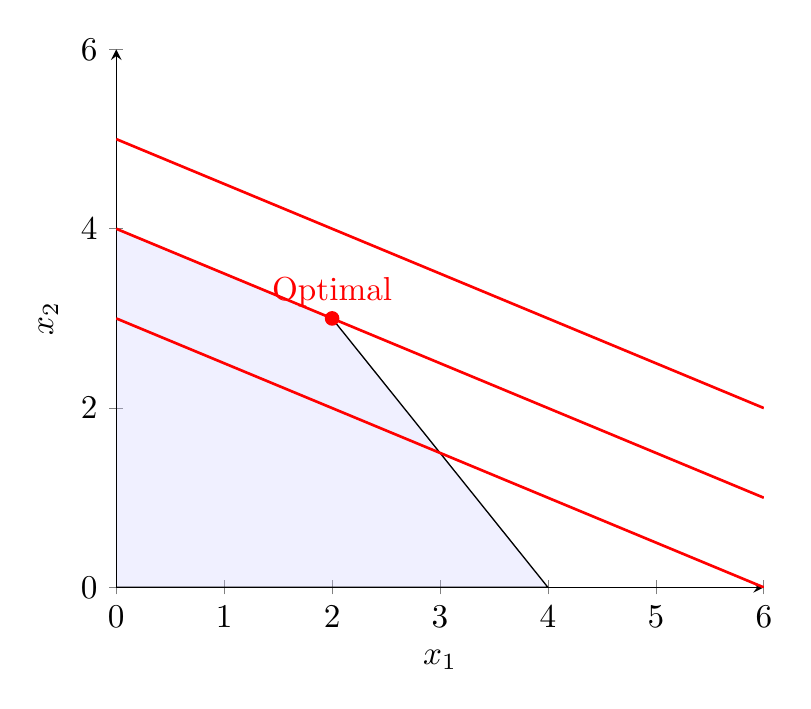
\begin{tikzpicture}[scale=1.2]
    \begin{axis}[
        axis lines = left,
        xlabel = $x_1$,
        ylabel = $x_2$,
        xmin=0, xmax=6,
        ymin=0, ymax=6,
    ]
    
    % Feasible region
    \addplot[fill=blue!20, fill opacity=0.3] coordinates {
        (0,0) (0,4) (2,3) (4,0) (0,0)
    };
    
    % Objective function contours
    \addplot[red, thick, domain=0:6] {3 - 0.5*x};
    \addplot[red, thick, domain=0:6] {4 - 0.5*x};
    \addplot[red, thick, domain=0:6] {5 - 0.5*x};
    
    % Optimal point
    \addplot[red, only marks, mark=*] coordinates {(2,3)};
    
    \node[red, above] at (2,3) {Optimal};
    
    \end{axis}
\end{tikzpicture}
\caption{Linear programming feasible region and objective contours}
\end{figure}

\section{Convex Optimization}

\subsection{Convex Sets}
\begin{definition}
A set $C \subseteq \mathbb{R}^n$ is \textbf{convex} if for all $x, y \in C$ and $\lambda \in [0,1]$:
$$\lambda x + (1-\lambda) y \in C$$
\end{definition}

\subsection{Convex Functions}
\begin{definition}
A function $f: C \to \mathbb{R}$ is \textbf{convex} if for all $x, y \in C$ and $\lambda \in [0,1]$:
$$f(\lambda x + (1-\lambda) y) \leq \lambda f(x) + (1-\lambda) f(y)$$
\end{definition}

\subsection{Convex Optimization Problem}
\begin{definition}
A convex optimization problem:
\begin{align}
\min \quad & f(x) \\
\text{s.t.} \quad & g_i(x) \leq 0, \quad i = 1, \ldots, m \\
& h_j(x) = 0, \quad j = 1, \ldots, p
\end{align}
where $f$ and $g_i$ are convex, and $h_j$ are affine.
\end{definition}

\subsection{Optimality Conditions}
\begin{theorem}[KKT Conditions]
For a convex optimization problem, $x^*$ is optimal if and only if there exist Lagrange multipliers $\lambda_i \geq 0$ and $\nu_j$ such that:
\begin{align}
\nabla f(x^*) + \sum_{i=1}^m \lambda_i \nabla g_i(x^*) + \sum_{j=1}^p \nu_j \nabla h_j(x^*) &= 0 \\
g_i(x^*) &\leq 0, \quad i = 1, \ldots, m \\
h_j(x^*) &= 0, \quad j = 1, \ldots, p \\
\lambda_i g_i(x^*) &= 0, \quad i = 1, \ldots, m
\end{align}
\end{theorem}

\section{Unconstrained Optimization}

\subsection{Gradient Descent}
\begin{definition}
Gradient descent for minimizing $f(x)$:
$$x_{k+1} = x_k - \alpha_k \nabla f(x_k)$$
where $\alpha_k$ is the step size.
\end{definition}

\subsection{Newton's Method}
\begin{definition}
Newton's method for optimization:
$$x_{k+1} = x_k - [\nabla^2 f(x_k)]^{-1} \nabla f(x_k)$$
\end{definition}

\subsection{Convergence Analysis}
\begin{theorem}
If $f$ is strongly convex with Lipschitz gradient, gradient descent with constant step size converges linearly:
$$f(x_k) - f(x^*) \leq \rho^k (f(x_0) - f(x^*))$$
for some $\rho < 1$.
\end{theorem}

\section{Constrained Optimization}

\subsection{Lagrange Multipliers}
\begin{definition}
For the problem $\min f(x)$ subject to $h(x) = 0$, the Lagrangian is:
$$L(x, \lambda) = f(x) + \lambda^T h(x)$$
\end{definition}

\subsection{Penalty Methods}
\begin{definition}
The penalty method approximates constrained problems by:
$$\min f(x) + \mu \sum_{i=1}^m [g_i(x)]_+^2 + \mu \sum_{j=1}^p h_j(x)^2$$
where $[z]_+ = \max(0, z)$.
\end{definition}

\subsection{Barrier Methods}
\begin{definition}
The barrier method uses:
$$\min f(x) - \mu \sum_{i=1}^m \log(-g_i(x))$$
for inequality constraints.
\end{definition}

\section{Integer Programming}

\subsection{Branch and Bound}
\begin{definition}
Branch and bound for integer programming:
\begin{enumerate}
    \item Solve LP relaxation
    \item If solution is integer, stop
    \item Branch on fractional variable
    \item Bound using LP relaxation
    \item Prune infeasible or suboptimal nodes
\end{enumerate}
\end{definition}

\subsection{Cutting Planes}
\begin{definition}
Cutting plane methods add valid inequalities to tighten the LP relaxation:
\begin{enumerate}
    \item Solve LP relaxation
    \item If solution is fractional, find cutting plane
    \item Add cut and resolve
    \item Repeat until integer solution
\end{enumerate}
\end{definition}

\section{Nonlinear Programming}

\subsection{Sequential Quadratic Programming}
\begin{definition}
SQP solves the subproblem:
\begin{align}
\min \quad & \frac{1}{2} d^T B_k d + \nabla f(x_k)^T d \\
\text{s.t.} \quad & \nabla g_i(x_k)^T d + g_i(x_k) \leq 0 \\
& \nabla h_j(x_k)^T d + h_j(x_k) = 0
\end{align}
where $B_k$ approximates the Hessian.
\end{definition}

\subsection{Trust Region Methods}
\begin{definition}
Trust region methods solve:
$$\min_{d: \|d\| \leq \Delta_k} m_k(d)$$
where $m_k(d)$ is a model of $f(x_k + d)$.
\end{definition}

\section{Stochastic Optimization}

\subsection{Stochastic Gradient Descent}
\begin{definition}
SGD for minimizing $E[F(x, \xi)]$:
$$x_{k+1} = x_k - \alpha_k \nabla F(x_k, \xi_k)$$
where $\xi_k$ is a random sample.
\end{definition}

\subsection{Robust Optimization}
\begin{definition}
Robust optimization considers uncertainty in parameters:
$$\min_{x} \max_{\xi \in \mathcal{U}} f(x, \xi)$$
where $\mathcal{U}$ is the uncertainty set.
\end{definition}

\section{Applications}

\subsection{Operations Research}
Optimization is used in:
\begin{itemize}
    \item Supply chain management
    \item Scheduling problems
    \item Resource allocation
    \item Network design
\end{itemize}

\subsection{Machine Learning}
Applications include:
\begin{itemize}
    \item Training neural networks
    \item Support vector machines
    \item Regularized regression
    \item Clustering algorithms
\end{itemize}

\subsection{Finance}
Used for:
\begin{itemize}
    \item Portfolio optimization
    \item Risk management
    \item Option pricing
    \item Algorithmic trading
\end{itemize}

\section{Important Theorems}

\subsection{Farkas' Lemma}
\begin{theorem}
Exactly one of the following holds:
\begin{enumerate}
    \item There exists $x \geq 0$ such that $Ax = b$
    \item There exists $y$ such that $A^T y \leq 0$ and $b^T y > 0$
\end{enumerate}
\end{theorem}

\subsection{Complementary Slackness}
\begin{theorem}
For optimal solutions $x^*$ and $y^*$ of primal and dual:
$$x_i^* > 0 \Rightarrow (A^T y^*)_i = c_i$$
$$(A^T y^*)_i < c_i \Rightarrow x_i^* = 0$$
\end{theorem}

\subsection{Minimax Theorem}
\begin{theorem}
For a convex-concave function $f(x,y)$:
$$\min_x \max_y f(x,y) = \max_y \min_x f(x,y)$$
\end{theorem}

\section{Complexity}

\subsection{Computational Complexity}
\begin{itemize}
    \item Linear programming: Polynomial time (interior point methods)
    \item Convex optimization: Polynomial time
    \item Integer programming: NP-hard
    \item General nonlinear programming: NP-hard
\end{itemize}

\subsection{Approximation Algorithms}
\begin{definition}
An $\alpha$-approximation algorithm produces a solution within factor $\alpha$ of optimal in polynomial time.
\end{definition}

\end{document}
